\documentclass[../uilmath.tex]{subfiles}
\graphicspath{{\subfix{../figures/}}}
\begin{document}
\chapter{Pre-Calculus}
\section*{Problems}
\begin{enumerate}[label=\bfseries\arabic*.]
    \item %% Problem 1
    The graph of $x^2+y^2-4x+12y+30=0$ is a circle with a diameter of: 

    \item %% Problem 2
    Let $\tan A = \frac{7}{24}$, where $A$ is in QIII. Find $\cos A$.

    \item %% Problem 3
    An equivalent expression for $(\sin x + \cos x)^2+(\sin x - \cos x)^2$ is:

    \item %% Problem 4
    The graph of $x^2+y^2+10x-12y-20=0$ is a circle with a radius of:

    \item %% Problem 5
    A cliff near a lake is 125 feet high. The angle of depression of a canoe from the top of the cliff is 30$\degree$. How far is the canoe from the base of the cliff? (nearest foot).

    \item %% Problem 6
    Simplify: $\sin\theta \tan\theta + \cos\theta$

    \item %% Problem 7
    Use the angle of rotation, $\theta$ (nearest degree), where 0$\degree<\theta<90\degree$, to transform the conic $xy=1$ into an equation that is in standard position and does not contain an $xy$ term. The transformed equation is:

    \item %% Problem 8
    The focus of the parabola below has coordinates $(a,b)$. $a+b=\blank$.
    \begin{center}
        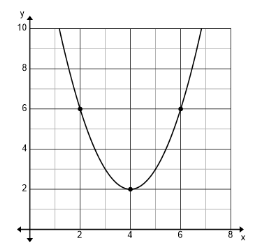
\includegraphics[width=0.3\textwidth]{2021SAC9.PNG}
    \end{center}

    \item %% Problem 9
    Find the eccentricity of the ellipse. $9x^2+16y^2-36x+96y+36=0$. (nearest hundredth)

    \item %% Problem 10
    Simplify: $4\csc(2x)\cos(x)$

    \item %% Problem 11
    Polonium 221 has a half-life of 130 seconds. How long will it take a sample with a mass of 1.80 g to decay to a mass of 1.20 g? (nearest tenth)

    \item %% Problem 12
    Assume the number of hours of daylight varies sinusoidally at the Clydehurst Christian Ranch in Montana. The longest day of the year has 15 hr 30 min of daylight and the 
    shortest day has 8 hr 30 min of daylight. How many days during the year have at least 13 hours of daylight?

    \item %% Problem 13
    The Holiday Inn is across the street from the Hilton. The hotels are 120 feet apart. Joe looks out the window of his room 
    at the Holiday Inn and notices that the angle of depression to the base of the Hilton is $36\degree$ and the angle of elevation 
    to the top of the Hilton is $44\degree$. How tall is the Hilton? (nearest foot)

    \item %% Problem 14
    The graph of $r=3-3\sin\theta$ is a \blank.

    \item %% Problem 15
    The graph of the parametric equations $x=2+3\cos\theta$ and $y=1+2\sin\theta$ is an ellipse with vertices 
    $(a,b)$ and $(c,b)$. $a+c=\blank$.

    \item %% Problem 16
    If $\frac{12i+8i^4+12i^3}{\sqrt{-100}+10i+6i^4}$ simplifies to $\frac{a}{b}+\frac{c}{b}i$, then $a+b+c=\blank$.

    \item %% Problem 17
    If $f(x)=\sec(2x)$ and $h(x)=\csc(3x)$. $f\left(\frac{5\pi}{8}\right)+h\left(\frac{11\pi}{18}\right)=\blank$. (nearest tenth)

    \item %% Problem 18
    Each of the wheels on Russell's jumbo wheel swamp buggy has a 4 ft diameter. When he is traveling 42 mph, what 
    is the angular velocity of the wheels in revolutions per minute? (nearest whole number)

    \item %% Problem 19
    The vertex of the parabola $y=-4x^2+6x-8$ is the point $(a,b)$. $a+b=\blank$. (nearest hundredth)

    \item %% Problem 20
    Multiply $(6\cis(60\degree))(-4\cis(-150\degree))$ and express the result in rectangular form.

    \item %% Problem 21
    Sarah released 36 bunnies into the woods near her house. Six months later the population had increased to 
    100 bunnies. Assume the bunny population is increasing exponentially and calculate the expected bunny population 21 months after the original release of 36 bunnies.

    \item %% Problem 22
    Devin drops a ball from a height of 24 feet. On each bounce, the ball rebounds three-fourths of the distance it fell. How far does the ball rebound on the tenth bounce? (nearest inch)

    \item %% Problem 23
    Consider $f(x)=x^3+bx^2+cx+d=0$. Two of the zeroes are $5$ and $2i$. $\mid b+c+d \mid=\blank$.

    \item %% Problem 24
    The vertices of the hyperbola $16y^2-9x^2-96y-72x-144=0$ are $(a,b)$ and $(a,c)$. $b+c=\blank$.

    \item %% Problem 25
    Consider a parabola with vertex $\left(\frac{3}{2},\frac{1}{4}\right)$. If the point 
    $(-2,4)$ lies on the graph of the parabola, which of the following points also lies on the graph of the parabola? The graph is concave up.

    $\textbf{(A)} (2,-2) \qquad \textbf{(B)} (3,0) \qquad \textbf{(C)} (4,2) \qquad \textbf{(D)} (5,4) \qquad \textbf{(E)} (6,6)$

    \item %% Problem 26
    Find the angle between the line $3x-y=6$ and the line $4x+5y=9$. (nearest tenth)

    \item %% Problem 27
    The graph of the polar equation $r=3-3\cos(\theta)$ is a $\blank$.

    \item %% Problem 28
    The graph of the parametric equations $x=13\cos(\theta)$ and $y=5\sin(\theta)$ is an ellipse with a foci $(a,b)$ and $(c,b)$. $\mid a-c \mid = \blank$.

    \item %% Problem 29
    Consider the sphere $x^2+y^2+z^2+4x-6y+2x-11=0$. Find the volume of the sphere. (nearest tenth)

    \item %% Problem 30
    The unit vector orthogonal to both $u=2i-3j+4k$ and $v=-2i+5j-7k$ is the vector 
    $\frac{a}{\sqrt{53}}i+\frac{b}{\sqrt{53}}j+\frac{c}{\sqrt{53}}k$. $a+b+c=\blank$.

    \item %% Problem 31
    

\end{enumerate}

\section*{Solutions}
\begin{enumerate}[label=\bfseries\arabic*.]
    \item %% Problem 1
    6.3 units 

    \item %% Problem 2
    $-\frac{24}{25}$

    \item %% Problem 3
    2

    \item %% Problem 4
    9

    \item %% Problem 5
    217 ft 

    \item %% Problem 6
    $\sec\theta$

    \item %% Problem 7
    $x^2-y^2=2$

    \item %% Problem 8
    $6\frac{1}{4}$

    \item %% Problem 9
    0.66

    \item %% Problem 10
    $2\csc(x)$

    \item %% Problem 11
    76.0 s 
    
    \item %% Problem 12
    148

    \item %% Problem 13
    203 ft

    \item %% Problem 14
    cardioid

    \item %% Problem 15
    4

    \item %% Problem 16
    81

    \item %% Problem 17
    -3.4

    \item %% Problem 18
    294 rpm 

    \item %% Problem 19
    -5.00 

    \item %% Problem 20
    24i

    \item %% Problem 21
    1286

    \item %% Problem 22
    16 in 

    \item %% Problem 23
    21

    \item %% Problem 24
    6

    \item %% Problem 25
    D 

    \item %% Problem 26
    69.8$\degree$

    \item %% Problem 27
    cardioid 

    \item %% Problem 28
    24

    \item %% Problem 29
    523.6

    \item %% Problem 30
    11

    \item %% Problem 31
    
\end{enumerate}

\end{document}